\chapter{Results and discussion}

You should have a separate chapter for presenting your results (generated by the stuff described previously, in our case in \cref{chap:math}). Remember that your work needs to be validated rigorously, and no one will believe you if you just say that `it worked well for you'.

Instead, try some of the following:
\begin{itemize}
\item State a hypothesis and prove it statistically
\item Show plots with measurements that you did to prove your results (e.g. speedup). Use either \texttt{R} and \texttt{ggplot}, or Python with \texttt{matplotlib} to generate the plots.\footnote{Honestly, the plots from \texttt{ggplot} look \underline{much} better.} Save them as PDF to avoid printing pixels (as in \cref{fig:f}).
\item Compare with other similar software/theses/authors/results, if possible
\item Show example source code (e.g. for demonstrating how easily your results can be used)
\item Include a `toy problem' for demonstrating the basic functionality of your approach and detail all important properties and results on that
\item Include clear pictures of `inputs' and `outputs' of all your algorithms, if applicable
\end{itemize}

\begin{figure}
\centering
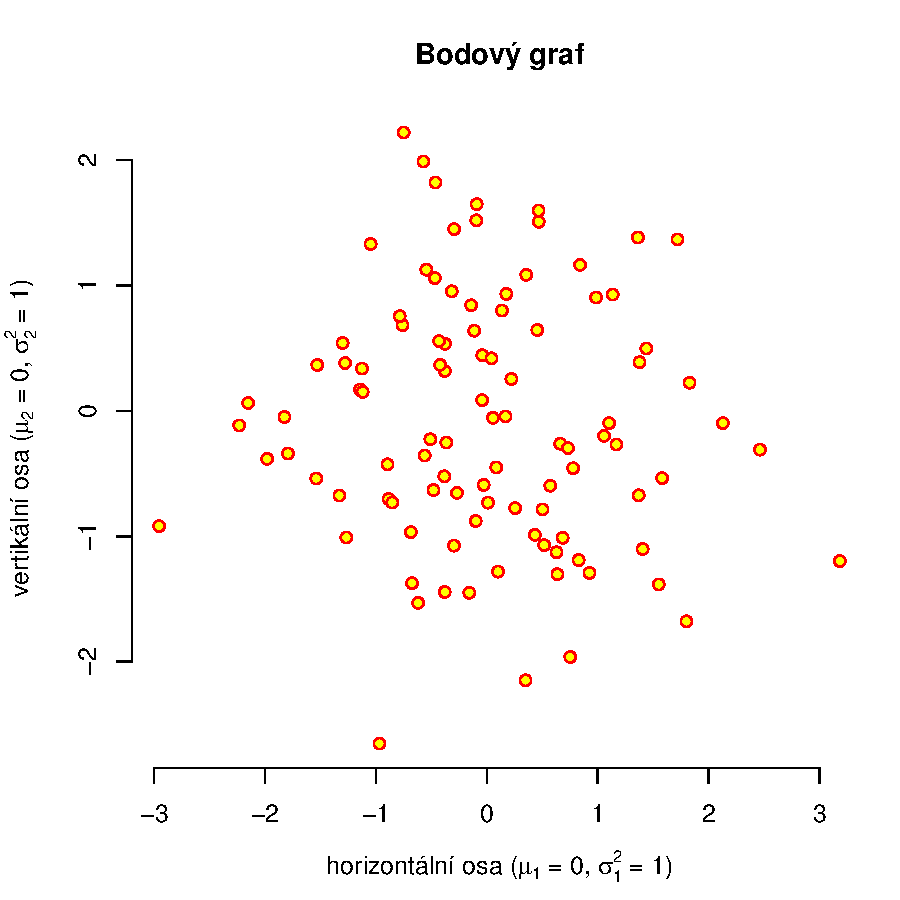
\includegraphics[width=.6\linewidth]{img/ukazka-obr01.pdf}
\caption{This caption is a friendly reminder to never insert figures ``in text,'' without a floating environment, unless explicitly needed for maintaining the text flow (e.g., the figure is small and developing with the text, like some of the centered equations, as in \cref{thm:y}). All figures \emph{must} be referenced by number from the text (so that the readers can find them when they read the text) and properly captioned (so that the readers can interpret the figure even if they look at it before reading the text --- reviewers love to do that).}
\label{fig:f}
\end{figure}

It is sometimes convenient (even recommended by some journals, including Cell) to name the results sub-sections so that they state what exactly has been achieved. Examples follow.

\section{SuperProgram is faster than OldAlgorithm}
\subsection{Scalability estimation}
\subsection{Precision of the results}
\section{Weird theorem is proven by induction}
\section{Amount of code reduced by CodeRedTool}
\subsection{Example}
\subsection{Performance on real codebases}
\section{\sloppy NeuroticHelper improves neural network learning}

\section{Graphics and figure quality}

No matter how great the text content of your thesis is, the pictures will always catch the attention first. This creates the very important first impression of the thesis contents and general quality. Crucially, that also decides whether the thesis is later read with joy, or carefully examined with suspicion.

Preparing your thesis in a way such that this first impression gets communicated smoothly and precisely helps both the reviewer and you: the reviewer will not have a hard time understanding what exactly you wanted to convey, and you will get a better grade.

Making the graphics `work for you' involves doing some extra work that is often unexpected. At the same time, you will need to fit into graphics quality constraints and guidelines that are rarely understood before you actually see a bad example. As a rule of thumb, you should allocate at least the same amount of time and effort for making the figures look good as you would for writing, editing and correcting the same page area of paragraph text.

\subsection{Visualize all important ideas}
The set of figures in your thesis should be comprehensive and complete. For all important ideas, constructions, complicated setups and results there should be a visualization that the reader can refer to in case the text does not paint the `mental image' sufficiently well. At the bare minimum, you should have at least 3 figures (roughly corresponding to the 3 chapters) that clearly and unambiguously show:
\begin{enumerate}
\item the context of the problem you are solving, optionally with e.g.~question marks and exclamation marks placed to highlight the problems and research questions
\item the overall architecture of your solution (usually as a diagram with arrows, such as in \cref{fig:schema}, ideally with tiny toy examples of the inputs and outputs of each box),
\item the advancement or the distinctive property of your solution, usually in a benchmark plot, or as a clear demonstration and comparison of your results.
\end{enumerate}

\subsection{Make the figures comprehensible}
The figures should be easily comprehensible. Surprisingly, that requires you to follow some common ``standards'' in figure design and processing. People are often used to a certain form of the visualizations, and (unless you have a very good reason) deviating from the standard is going to make the comprehension much more complicated. The common standards include the following:
\begin{itemize}
  \item caption everything correctly, place the caption at an expectable position
  \item systematically label the plots with `main' titles (usually in boldface, above the plot), plot axes, axis units and ticks, and legends
  \item lay out the diagrams systematically, ideally follow a structure of a bottom-up tree, a left-to-right pipeline, a top-down layered architecture, or a center-to-borders mindmap
  \item {use colors that convey the required information correctly \par\footnotesize Although many people carry some intuition for color use, achieving a really correct utilization of colors is often very hard without previous experience in color science and typesetting. Always remember that everyone perceives color hues differently, therefore the best distinction between the colors is done by varying lightness of the graphics elements (i.e., separating the data by dark vs.~light) rather than by using hues (i.e., forcing people to guess which one of salmon and olive colors means ``better''). Almost 10\% of the population have their vision impaired by some form of color vision deficiency, most frequently by deuteranomaly that prevents interpretation of even the most `obvious' hue differences, such as green vs.~red. Finally, printed colors look surprisingly different from the on-screen colors. You can prevent much of these problems by using standardized palettes and well-tested color gradients, such as the ones from ColorBrewer\footnote{\url{https://colorbrewer2.org}} and ViridisLite\footnote{\url{https://sjmgarnier.github.io/viridisLite/}}. Check if your pictures still look good if converted to greyscale, and use a color deficiency simulator to check how the colors are perceived with deuteranomaly.}
\end{itemize}

Avoid large areas of over-saturated and dark colors:
\begin{itemize}
  \item under no circumstances use dark backgrounds for any graphical elements, such as diagram boxes and tables --- use very light, slightly desaturated colors instead
  \item avoid using figures that contain lots of dark color (as a common example, heatmaps rendered with the `magma' color palette often look like huge black slabs that are visible even through the paper sheet, thus making a dark smudge on the neighboring page)
  \item increase the brightness of any photos to match the average brightness of the text around the figure
\end{itemize}

Remember to test your figures on other people --- usually, just asking `What do you think the figure should show?' can help you debug many mistakes in your graphics. If they think that the figure says something different than what you planned, then most likely it is your figure what is wrong, not the understanding of others.

Finally, there are many magnificent resources that help you arrange your graphics correctly. The two books by Tufte~\cite{tufte1990envisioning,tufte1983visual} are arguably classics in the area. Additionally, you may find many interesting resources to help you with technical aspects of plotting, such as the \texttt{ggplot}-style `Fundamentals' book by~\citet{wilke2019fundamentals}, and a wonderful manual for the TikZ/PGF graphics system by~\citet{tantau2015tikz} that will help you draw high-quality diagrams (like the one in~\cref{fig:schema}).

\section{What is a discussion?}
After you present the results and show that your contributions work, it is important to \emph{interpret} them, showing what they mean in the wider context of the thesis topic, for the researchers who work in the area, and for the more general public, such as for the users.

Separate discussion sections are therefore common in life sciences where some ambiguity in result interpretation is common, and the carefully developed intuition about the wider context is sometimes the only thing that the authors have. Exact sciences and mathematicians do not need to use the discussion sections as often. Despite of that, it is nice to position your output into the previously existing environment, answering:
\begin{itemize}
\item What is the potential application of the result?
\item Does the result solve a problem that other people encountered?
\item Did the results point to any new (surprising) facts?
\item How (and why) is the approach you chose different from what the others have done previously?
\item Why is the result important for your future work (or work of anyone other)?
\item Can the results be used to replace (and improve) anything that is used currently?
\end{itemize}

If you do not know the answers, you may want to ask the supervisor. Also, do not worry if the discussion section is half-empty or thoroughly pointless; you may remove it completely without much consequence. It is just a bachelor thesis, not a world-saving avenger thesis.
